\chapter{Domaines de l'informatique concernés}
\label{chap:domaines}

Notre projet relève de plusieurs domaines informatiques.
\newline
Premièrement, l'algorithmique. En effet, l'algorithmique est l'étude et la production d'un ensemble de règles opératoires, présent dans ce qu'on appelle un algorithme, dont l'application permet de résoudre un problème énoncé au moyen d'un nombre fini d'opérations. Ainsi, avant de commencer la programmation, nous avons réfléchi à des algorithmes permettant de nous aider à savoir comment le programmer mais aussi d'avoir une meilleure idée de comment notre code fonctionnera. C'est à ce moment-là que nous avons réfléchi à comment modéliser les données de notre problème. Au tout début, nous avons donc réfléchi en jouant au casse-tête s'il existait un moyen d'optimiser notre façon de résoudre le Hashi afin d'être plus rapide et dans le but de réaliser le meilleur temps entre nous. Ainsi, nous avons commencé par écrire, au brouillon, des algorithmes contenant des conditions et des boucles de manière à trouver ce qu'on appellera plus tard des règles qui nous permettent de détecter les cas les plus triviaux et, à partir de là, d'élucider le reste du casse-tête de façon plus simple. 
\smallbreak
Deuxièmement, la programmation objet, car c'est avec le langage C++ que nous avons décidé de travailler, et c'est avec des objets que nous représentons ces données. Ce langage va nous permettre de pouvoir modéliser notre problème et donc de pouvoir y travailler concrètement dessus (Figure 1.1). Le langage C++ nous étant imposé, nous n'avons pas eu à avoir le choix parmi les autres langages objets existant, cependant, ceci ne nous dérangeait absolument pas du fait que nous préférions ce langage à d'autres langages qui nous étaient moins connus. En effet, parmi les centaines de langages de programmation qui existent, certains sont plus populaires que d'autres. Sans aucun doute, le C++ est un langage très populaire et c'est principalement pour cela que nous l'avons à apprendre au cours de notre cursus. La popularité n'est pas le seul critère de ce dernier puisque c'est en effet un langage puissant et particulièrement rapide le rendant essentiel pour le développement de jeux par exemple. Ainsi, pour résumer grossièrement, nous pouvons dire qu'il est très répandu, aidant ainsi la compréhension de ce dernier puisque nous pouvons obtenir de l'aide plus aisément, qu'il est rapide, utilisé pour des applications qui ont besoin de performances et qu'il est portable sur toutes les plates-formes telles que Windows, Mac OS et Linux.\newline

\begin{figure}[htp]
  \centering
  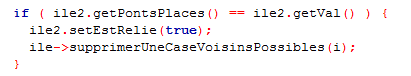
\includegraphics[width=13cm]{images/exemplec++}
  \caption{Exemple de code en C++}
\end{figure}
